\documentclass{beamer}
\usetheme{Madrid}
\usepackage[T1]{fontenc}
\usepackage{mathpazo}
\usepackage{graphicx}
\usepackage{booktabs}
\usepackage{tikz}
\usetikzlibrary{positioning,arrows.meta,shapes.geometric,fit,backgrounds,calc}
\definecolor{cetnavy}{RGB}{10,26,63}
\definecolor{cetlight}{RGB}{225,231,242}
\setbeamercolor{structure}{fg=cetnavy}
\setbeamercolor{frametitle}{bg=cetnavy,fg=white}
\setbeamercolor{title}{bg=cetnavy,fg=white}
\setbeamertemplate{navigation symbols}{}
% =====================================================================
%  EDIT YOUR DETAILS HERE — this ONE file feeds every abstract & deck.
%  (Change a value, recompile; all 36 documents update.)
% =====================================================================
\newcommand{\seminarName}{Aflah Muhammed P}      % <-- your full name (guessed from your email; please verify)
\newcommand{\seminarRoll}{TVE00CS000}            % <-- your university register/roll number
\newcommand{\seminarClassRoll}{00}               % <-- your class roll no (the short one)
\newcommand{\seminarGuide}{Prof.\ <Guide Name>}  % <-- your guide
\newcommand{\seminarDept}{Department of Computer Science and Engineering}
\newcommand{\seminarCollege}{College of Engineering Trivandrum}
\newcommand{\seminarShortCollege}{CET}           % shown in the slide footer, e.g. "Aflah Muhammed P (CET)"
\newcommand{\seminarShortTitle}{B.Tech Seminar}  % middle of the slide footer
\newcommand{\seminarDate}{July 31, 2026}
% ---------------------------------------------------------------------
% Optional: put a logo image named  cet_logo.png  in this folder and it
% will appear on every title slide automatically. If absent, it is skipped.
% =====================================================================

\title[\seminarShortTitle]{Multi-Agent Debate for Equitable Cultural Alignment}
\author[\seminarName\ (\seminarShortCollege)]{\seminarName \\ \seminarRoll \\ Roll No: \seminarClassRoll \\ Guide: \seminarGuide}
\institute[\seminarShortCollege]{\seminarDept \\ \seminarCollege}
\date{\seminarDate}
\titlegraphic{\IfFileExists{cet_logo.png}{\includegraphics[height=1.1cm]{cet_logo.png}}{}}
\begin{document}
\begin{frame}\titlepage\end{frame}
\begin{frame}{Table of Contents}\tableofcontents\end{frame}
\section{Introduction}
\begin{frame}{Cultural alignment of LLMs}
\begin{itemize}
\item LLMs now serve users across many cultures.
\item They align best with Western, high-resource norms.
\item Everyday etiquette varies sharply by country.
\item Equitable cross-cultural behaviour stays unsolved.
\end{itemize}
\end{frame}

\begin{frame}{This work in one line}
\begin{itemize}
\item Let two LLM agents \textit{debate} a scenario.
\item Agents jointly decide if behaviour is acceptable.
\item Debate lifts accuracy \emph{and} cross-country fairness.
\end{itemize}
\end{frame}

\section{Literature Survey}
\begin{frame}{Related work}
\textbf{\textit{Cultural evaluation}}
\begin{itemize}
\item NormAd benchmarks measure cultural adaptability.
\item Prompting and fine-tuning inject cultural values.
\end{itemize}
\textbf{\textit{Multi-agent and reflection}}
\begin{itemize}
\item Multi-agent debate aids reasoning and factuality.
\item Self-reflection lets a model self-correct.
\item Fairness across cultures remains under-studied.
\end{itemize}
\end{frame}

\section{Motivation}
\begin{frame}{Why debate?}
\begin{itemize}
\item One model encodes skewed cultural priors.
\item Prompting alone gives uneven, country-specific gains.
\item Different LLMs cover different cultural regions.
\item Debate can pool their complementary strengths.
\end{itemize}
\end{frame}

\section{Problem Statement}
\begin{frame}{The task}
\begin{itemize}
\item Judge etiquette scenarios from 75 countries.
\item Predict acceptability: Yes / No / Neither.
\item Maximise accuracy \emph{and} cross-country parity.
\item Avoid favouring dominant cultural groups.
\end{itemize}
\end{frame}

\section{Objectives}
\begin{frame}{Goals of the paper}
\begin{itemize}
\item Design multi-agent debate for cultural judgement.
\item Compare debate vs single-LLM and self-reflection.
\item Measure both accuracy and group parity.
\item Test if small models rival large ones.
\end{itemize}
\end{frame}

\section{Methodology Overview}
\begin{frame}{Debate pipeline}
\begin{center}
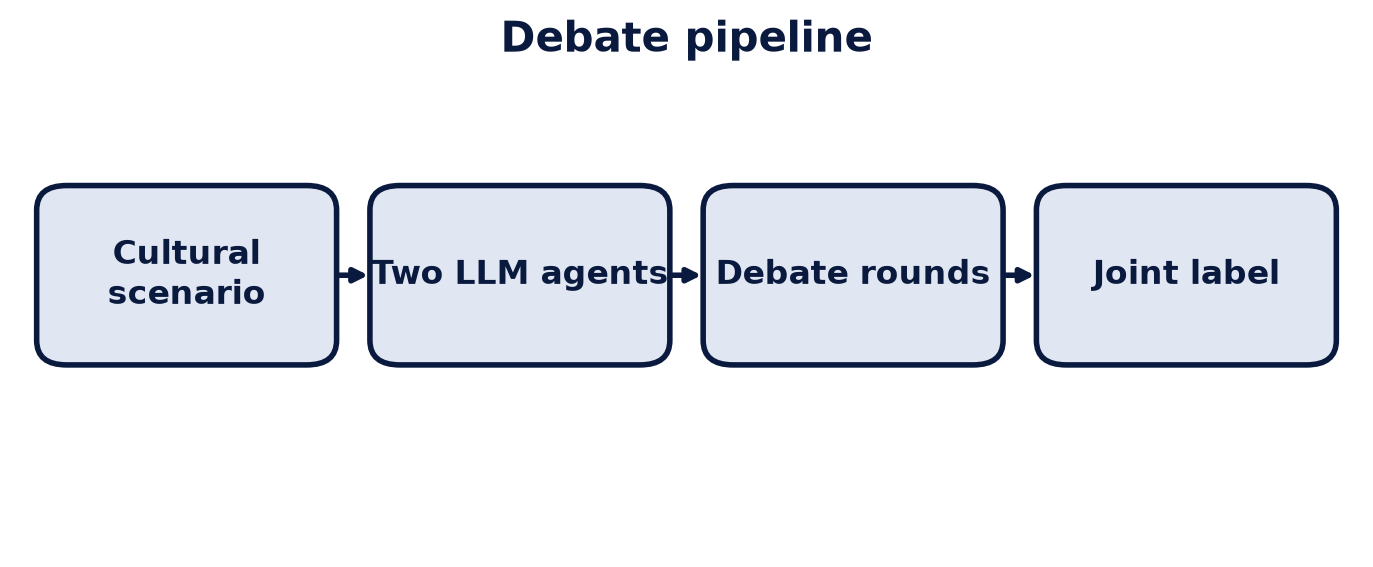
\includegraphics[width=0.9\textwidth,height=0.62\textheight,keepaspectratio]{images/culturaldebate_1.png}
\end{center}
\begin{itemize}
\item Each agent argues, then they converge on one label.
\end{itemize}
\end{frame}

\section{System Architecture}
\begin{frame}{Framework components}
\begin{center}
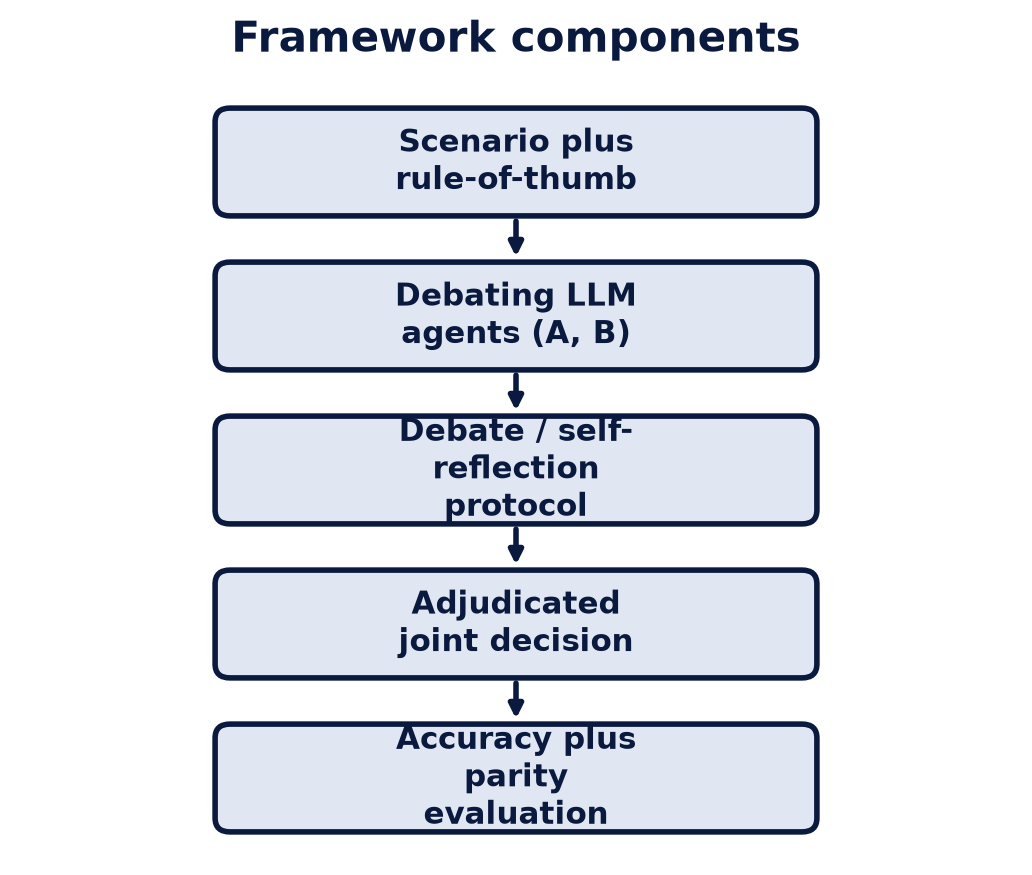
\includegraphics[width=0.9\textwidth,height=0.62\textheight,keepaspectratio]{images/culturaldebate_2.png}
\end{center}
\end{frame}

\section{Data Collection}
\begin{frame}{NormAd-ETI benchmark}
\begin{itemize}
\item About 2.6K social etiquette stories.
\item Drawn from the Cultural Atlas, 75 countries.
\item Each: country, rule-of-thumb, gold label.
\item Ternary labels: Yes / No / Neither.
\item Countries grouped by Inglehart-Welzel cultural map.
\end{itemize}
\end{frame}

\section{Model Development}
\begin{frame}{Turn-level action choice}
\begin{center}
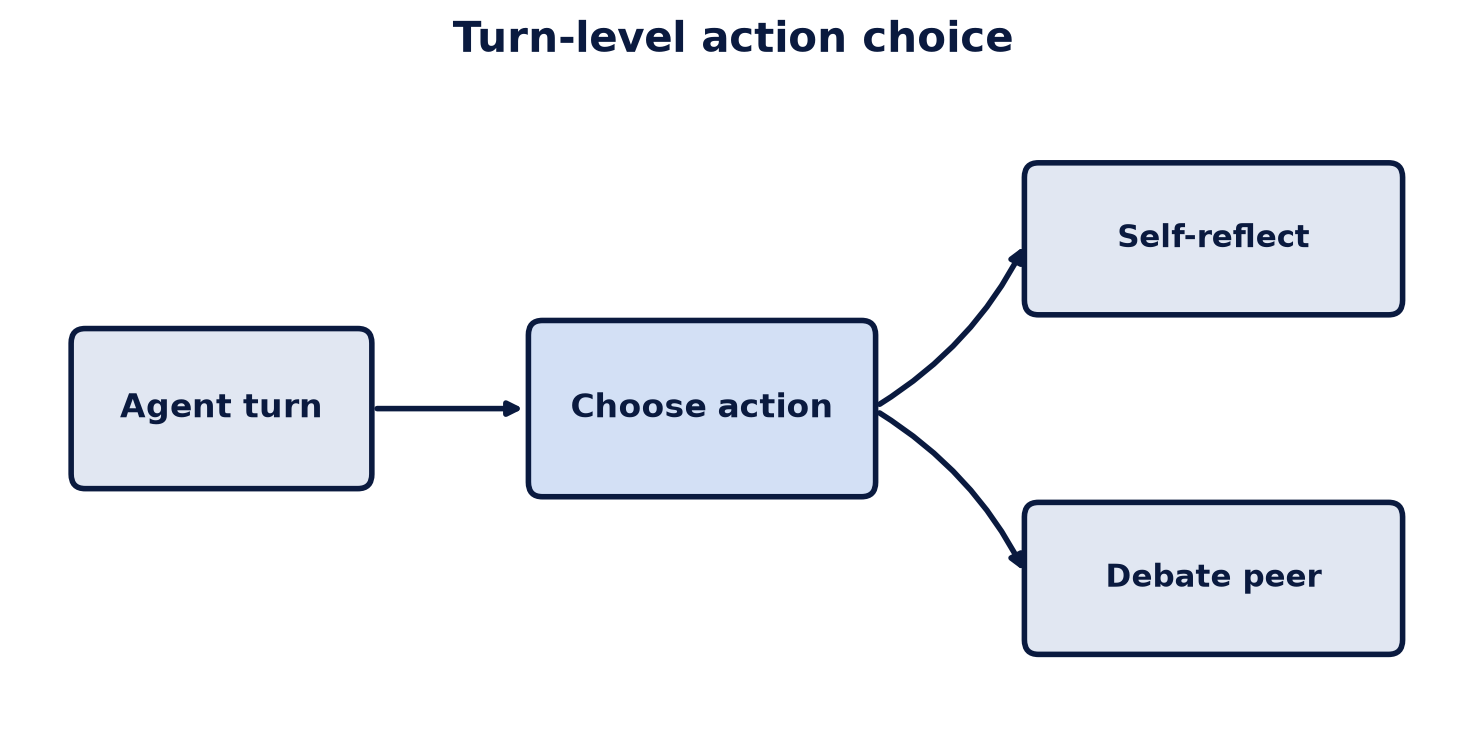
\includegraphics[width=0.9\textwidth,height=0.62\textheight,keepaspectratio]{images/culturaldebate_3.png}
\end{center}
\begin{itemize}
\item Self-Reflect+Debate picks an action each turn.
\end{itemize}
\end{frame}

\begin{frame}{Methods compared}
\textbf{\textit{Baselines}}
\begin{itemize}
\item Single LLM, with or without rule-of-thumb.
\item Iterative self-reflection.
\end{itemize}
\textbf{\textit{Proposed debate}}
\begin{itemize}
\item Debate-Only: two agents exchange arguments.
\item Self-Reflect+Debate: dynamic action per turn.
\item 7 open-weight LLMs, 21 pairings.
\end{itemize}
\end{frame}

\section{Results}
\begin{frame}{Main trends}
\begin{center}
\begin{tabular}{lcc}
\toprule
Method & Accuracy & Group parity \\
\midrule
Single LLM & baseline & baseline \\
Self-reflection & modest & mixed \\
Debate-Only & $\uparrow$ & $\uparrow$ \\
Self-Reflect+Debate & $\uparrow\uparrow$ & $\uparrow$ \\
\bottomrule
\end{tabular}
\end{center}
\begin{itemize}
\item Debate raises accuracy \emph{and} cross-country parity.
\item Small 7--9B models rival a 27B model.
\end{itemize}
\end{frame}

\section{Discussions}
\begin{frame}{Why it works}
\begin{itemize}
\item Peer critique corrects cultural blind spots.
\item Complementary models jointly cover more cultures.
\item Debate acts as test-time ensembling.
\item Gains arrive without extra fine-tuning.
\end{itemize}
\end{frame}

\section{Challenges}
\begin{frame}{Limitations}
\begin{itemize}
\item Adjudicating persistent agent disagreement is hard.
\item Debate adds inference-time cost.
\item Benchmark covers etiquette, not all norms.
\item Parity improves but stays imperfect.
\end{itemize}
\end{frame}

\section{Future Work}
\begin{frame}{Directions}
\begin{itemize}
\item Assign explicit roles to agents.
\item Develop better adjudication and voting.
\item Scale beyond two debating agents.
\item Extend to more languages and domains.
\end{itemize}
\end{frame}

\section{Conclusion}
\begin{frame}{Takeaways}
\begin{itemize}
\item Multi-LLM debate improves cultural alignment.
\item It boosts accuracy and fairness together.
\item Small models can rival much larger ones.
\item A promising path to equitable alignment.
\end{itemize}
\end{frame}

\section{References}
\begin{frame}{References}
\footnotesize
\begin{itemize}
\item D. Ki, R. Rudinger, T. Zhou, and M. Carpuat, ``Multiple LLM Agents Debate for Equitable Cultural Alignment,'' in Proc. ACL, 2025, arXiv:2505.24671.
\item A. Rao et al., ``NormAd: A Benchmark for Measuring the Cultural Adaptability of Large Language Models,'' arXiv:2404.12464, 2024.
\item Y. Du et al., ``Improving Factuality and Reasoning in Language Models through Multiagent Debate,'' arXiv:2305.14325, 2023.
\end{itemize}
\end{frame}
\begin{frame}\vfill\centering{\Huge Thank You}\vfill\end{frame}
\end{document}
